\chapter{Network Structure of Science} \label{Network Structure of Science}

De Solla's seminal paper \cite{deSollaPrice510} begins like this: \textit{"This article is an attempt to describe in the broadest outline the nature of the total world network of scientific papers. We shall try to picture the network which
is obtained by linking each published paper to other papers directly associated with it."}. Already at the beginning of the study of scientometrics it appeared evident that
science needed to be tackled from a global perspective, analyzing the connections that link scientific papers to one another.
 Similarly, two co-authors of the same paper
can be linked together, as well as two scientists who have collaborated with the same scientist as the famous Erd\H{o}s number grasps \cite{10.2307/2317868} 
\footnote{The Erd\H{o}s number measures the distance in terms of collaborative steps between the Hungarian mathematician Erd\H{o}s and his direct or indirect collaborators. Anyone
who has collaborated with him has a Erd\H{o}s number equal to 1. All their collaborators have a EN of 2 and so on.}. In general, the 
intrinsic collaborative nature of science either by cumulative contribution (the shoulders of giants) or by direct collaboration has led to the creation of a massive
scientific network that can be analyzed in many of its levels, where both its nodes and links can take many forms, with nodes representing papers as well as authors, institutions or countries and links representing
citations, co-authorship, shared funding etc. 

Graph theory showed for the first time the potential of network research for practical problems in the famous work by Euler in 1796; by simplifying the bridge and road structure of the
city of K{\"o}nigsberg in terms of nodes (land masses) and links (bridges), the Swiss mathematician was able to negatively answer the question: is it possible to perform a path around the city that
crosses each bridge of the city exactly once? For a long time graph (or network) theory remained confined mainly as a branch of topology in theoretical mathematics \cite{Cayley1881} until the middle
of the 19th century when the earliest structured books appeared  \cite{0817633898,9782746232150}, allowing the developments in the theory to spread
to new fields \cite{0123242509}, including sociology, where researchers understood that a matrix based representation, i.e. one of the underlying bedrocks of network theory,
of social ties could be beneficial for the study of social structures \cite{Luce1949,10.2307/2088670}. The breakthrough came in 1959 with Erd\H{o}s and R\'{e}nyi's work on
random graphs \cite{citeulike:4012374} in which the authors studied
the invariant properties of graphs generated through a stochastic model that distributes a fixed number of links across all possible node pairs. The ER model turned out to have strong
analogies with statistical mechanics \cite{COHEN1988113} and was later used as a fundamental tool for studies that required a network based structure, in particular 
for models in epidemiology \cite{pmid7608641,Keeling859}. 

In general, the ER model allowed the rise of what are called \textit{generative models}. 
These models aim at reproducing the statistical properties of the observed networks \cite{1608.00607}, yet keeping the most important features (usually
the degree distribution or the average degree) of the network
statistically constant, while allowing for the edges to be distributed at random. Generative models therefore act as tools for generating null-hypothesis that can be tested statistically,
allowing to identify which properties in real networks are statistically relevant, with applications to multiple fields \cite{Connor1979,Gail1977}. Among the attempts, de Solla Price
contributed with the earliest definition of the rich get richer mechanism \cite{Price1976} that would later be made popular by Barab{\'a}si and Albert, who
showed its potential \cite{Barabasi509} as a tool to describe the emergence of scale-free networks. Barab{\'a}si and Albert's paper was part of a period
of extreme interest for network theory studies as the rapid accumulation of data of large networks thanks to the digitalization of society, allowed
for the first time to provide a robust set of data that could be used to test previous models. While the ER model had been extremely successful due to 
its simplicity, the evidence of different properties in real networks required the development of new models, which rapidly took place \cite{Watts1998,Albert2002}


Since then, network theory has been applied in a large spectrum of fields, dealing with non-trivial network structures that required methods and algorithms tailored to specific types of network problems, leading to a whole new field, often referred to as \textit{complex networks}, in order to differentiate it from Graph Theory. As the theory developed,
the application of its methods to publication data became a fertile branch of the field. 
This Chapter will first go through the basics of network theory, in order to provide a mathematical foundation for the rest of the chapter, in which the most significant
applications to scientific networks will be discussed.

\section{Networks}
A network, also called graph, is a collection of nodes connected by links. Mathematically it is represented
by $G = (V, E)$ where $V$ is a set of $N$ nodes and $E$ is a set of $M$ links (or edges) connecting pairs of nodes. 
A convenient way to represent a network is through its \textit{adjacency matrix} $A$, which fully describes the graph.  Its
elements $a_{ij}$ are 1 if there is a link connecting node i and node j and 0 otherwise. If
$A$ is symmetric the graph is undirected as all of its links go in both directions. It is often assumed that there are no self loops, i.e. $a_{ii}=0$
for all i. In this simplest scenario, the elements of the matrix are usually binary and symmetric, thus only indicating whether two nodes have a connection or not.
However, more sophisticated networks can be built by modifying these conditions:
\textit{Directed graphs} take into account the directionality of the links by dropping the symmetry requirement, while \textit{weighted} graphs drop the binary requirement
for the elements of the matrix, thus quantifying the "strength" of the link. An example are mobile call networks, in which $a_{ij}$ can indicate the number
of calls between user $i$ and $j$, or the total time spent between two users \cite{Onnela01052007}. Networks in which most elements of the adjacency matrix
are 0s are usually called \textit{sparse}, while in the opposite case they are called \textit{dense}. Sparse matrices, which
are not rare at all \cite{Davis:2011:UFS:2049662.2049663}, can represent a problem computationally
in terms of storage space since, if stored in matrix form, $N^{2}$ entries need to be stored, most of which do not carry information.
Fortunately, the disadvantage can be turned in an advantage by using \textit{adjacency lists} in which each row $i$ enumerates
the neighbors of the node along with the value of the edge in case it is required. 
Recently, there has been a need to analyze many different kinds of network structures. For example, temporal networks take into consideration the intermittent activity of the edges in the network, thus adding 
a temporal dimension to the analysis of complex networks \cite{Holme201297}. Multilayer networks instead deal with
systems in which nodes exist in one or more of multiple layers and where links can connect nodes also across layers \cite{Kivela2014,Boccaletti2014}.
Such networks can be useful to analyze interactions in social systems, where each layer represents a different kind of interaction and where
not all users are equally active in each layer, or might not be active at all in some of them \cite{Szell03082010}.




\subsection{Degree}
The degree $k_{i}$ of a node is the number of nodes that node i is connected to. 
It can be derived using the adjacency matrix $A$ as  $k_{i} = \sum_{j} a_{ij} $, i.e. the sum of the nonzero elements of
row $i$. In case of a directed network two separate degrees are considered : $k^{in}_{i}$ and $k_{i}^{out}$, which differentiate
between the degree calculated respectively over the columns or the rows. The average degree  $\bar{k}$  of a network is the average value of individual degrees 
  $\bar{k} = \frac{\sum_{i} k_{i}}{N} $, where $N$ is the number of nodes in the network. Again, it is possible to define an average $\bar{k}^{in}_{i}$ and $\bar{k}_{i}^{out}$ for directed networks.
  
When analyzing a large network, it can be useful to look at the overall distribution of the degree values for the nodes of the network, as with an increasing number of nodes it 
becomes necessary to analyze them statistically. In the ER model \footnote{This formulation was presented in the same year by Gilbert \cite{gilbert1959} and is statistically equivalent
to the ER model.} each link exists with probability $\frac{M}{\binom{N}{2}}$, leading to the probability of node $i$ to have degree $k$ to be the 
probability of having $k$ times successful
Bernoulli trials, thus converging to a Poissonian distributions as the size of the network grows, with $\bar{k}$ remaining constant.
However, empirical evidence \cite{Barabasi2004degree}
has shown that real world networks have a dramatically different behaviour when it comes to degree distribution.

While the ER model predicts a large amount of nodes sharing
similar degree values, social, biological and transportation network among others, revealed themselves to have fat-tailed distributions \cite{Clauset2009}, i.e. they showed the existence of nodes with large degree called \textit{hubs}, along with a 
vast amount of nodes with low degree values. In 1999, Barab{\'a}si and Albert proposed a different model, in which the network is generated by adding new nodes and
connecting
them proportionally to the degree of the previously existing nodes, through the Preferential Attachment Method already introduced in the previous chapter. In Fig.\ref{fig:degree} we can see a comparison
between the appearance and the degree distribution of a random networks compared to a scale-free network. 
 \begin{figure}[h]
\centering
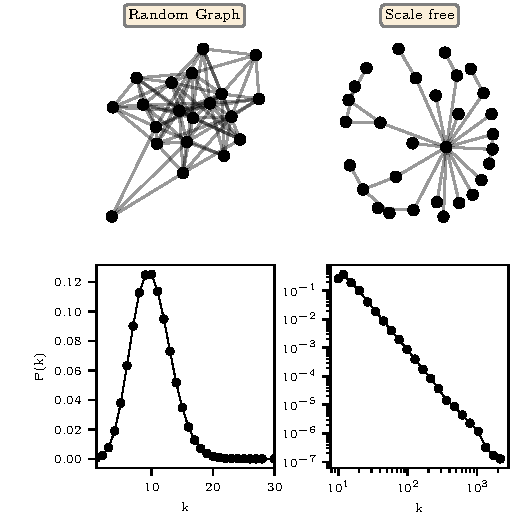
\includegraphics[width=.8\textwidth]{degree_histogram.pdf}%
\caption{Difference in topology and degree distribution between a random graph (left) and a scale-free network (right). The random network has its degree distribution heavily
centered around its average, with no significant outliers. In the scale-free model instead, degrees can span multiple orders of magnitude.}
\label{fig:degree}
\end{figure}
   
Another fundamental property of degree  is linked to the concepts of \textit{assortativity} and \textit{resilience}. Assortativity is used to investigate what is the tendency in a network for nodes with similar 
degree to be connected \cite{PhysRevLett.89.208701,Newman2003} and is therefore often expressed as degree-degree correlation. In a network with high assortativity, high-degree nodes are likely to be connected
and tend to avoid connections to low-degree nodes. Similarly, a network is disassortative if high degree nodes tend to avoid being linked to each other and prefer being connected to lower
degree nodes. In both the ER and Preferential Attachment models, there is no correlation between degrees; in the ER model
links are given randomly, thus an absence of correlation is to be expected for large graphs, while in the PA model the evidence is less trivial, but it comes from the fact that hubs have a tendency to get links
from all new nodes, thus failing to select connections to specific nodes. Interestingly, real life networks show different scenario, with certain networks being assortative (power grids, social networks) and other disassortative (WWW, protein-interaction
networks), thus requiring more sophisticated models to be able to reproduce these features \cite{Callaway2001}. A direct consequence of assortativity is resilience, i.e. the ability of a network to resist
the attack or failure of random nodes. In a air transportation network for example, this corresponds at how the passenger traffic is affected by the closure of randomly selected airports. Numerical simulations \cite{PhysRevLett.89.208701}
show that a high assortativity is linked to a better chance to resist attacks due to the fact that hubs, which are often fundamental as they allow to distribute "services" to the periphery of the network, are likely to be connected
to each other, thus creating dense cores of highly connected nodes that keep the structure of the network efficient. In disassortative networks instead, hubs are fundamental local service providers and, if shut down,
are more likely to cause an interruption in services. Unfortunately, many communication networks are disassortative \cite{doi:10.1093/comnet/cnv005} and have therefore been often
subject of systematic failures \cite{Sterbenz20101245} due to their structural inefficiency.


\subsection{Clustering, paths and distances}
The clustering coefficient measures how likely two nodes within the neighbourhood of a node are also
 be connected \cite{Watts1998}. Let's consider a node with $k$ neighbours. Among these neighbours there are $\frac{k(k-1)}{2}$ possible links, i.e. the number of ways 2 nodes can be selected if there are k nodes,
 out of which only $E_{i}$ are present in the network. The CC is defined as the ration between the two terms:
\begin{equation}
 C_{i} = \frac{E_{i}}{\frac{k_{i}(k_{i} -1)}{2}}
\end{equation}
In case of weighted and directed graphs the concept can be generalized 
in multiple ways \cite{Fagiolo2007}. The average clustering coefficient of a network is the average $C = \sum_{i} C_{i}/ N$ of the individual clustering coefficients.
 The global clustering coefficient is a similar measure as the average clustering coefficient which looks 
at the clustering of a network from a geometric point of view. It is defined as the fraction of triplets (i.e. a set of 3 connected nodes) that actually form a triangle and can be applied to both undirected and directed networks \cite{Newman2003Complex}.
In an undirected network the average path length between two nodes is defined as $l = \frac{1}{\frac{n(n+1)}{2}} \sum_{i\geq j} d_{ij}$,
where $d_{ij}$ is the length of the shortest path between two nodes. In case the graph is not connected (i.e. there are parts of the networks that are separated), the value of the average path length diverges and is therefore
convenient to compute it individually for each subgraph of the network. The diameter, $D$, of a network is defined as the maximum shortest path between any two nodes in the network. Its name recalls the topologic
properties of circles as it represents the approximate linear size of the network.  

In 1998 Watts and Strogatz published a paper that showed how the currently available models based either on regular lattices or on random graphs were unable to grasp the properties of real networks in terms of clustering coefficient
and path length\cite{Watts1998}. While their analysis of diverse networks (power grids, biological networks, film actors) showed large CC and short paths, the ER model  \cite{Albert2002} is bound to generate networks
with average path length $\propto log(N)$ and have an extremely low value for the CC. They called their networks \textit{small-world networks} in reference to the famous social experiment of the six degrees
of separation \cite{sixdeg}, which was the first attempt at calculating path lengths in social networks. They proposed a stylized model based on a regular lattice, thus guaranteeing high clustering, with a random rewiring
of each link controlled by a parameter $p$. The value of $p$ therefore allows the transition from a regular lattice ($p=0$) to a random network $p=1$. As $p$ increases from 0, local clustering remains high while
paths between distant nodes cause a significant reduction of the average path lengths. With this simple model Watts and Strogatz managed to show how even a small number of short cuts
can transform a sparse, locally clustered network in a small-world one.


\subsection{Communities and modularity}
Between 1970 and 1972 Wayne W. Zachary collected data about the interaction between 34 members of a karate club, during which two instructors had an argument, leading to a split of the group into two, with half of the group
remaining in the club with one instructor and the other half leaving it  \cite{10.2307/3629752}. Based on the difference between the interaction patterns, Zachary was able to devise an algorithm able to automatically
detect in which half a node would lie. This became the first example, and later the benchmark, of a \textit{community detection} algorithm \cite{Fortunato201075}. The idea behind community detection is that networks can be organized in locally highly connected clusters separated one from the other, known as communities. Real world examples are abundant:
metabolic networks are organized into small, highly connected modules \cite{Ravasz2002}, urban areas and societies can be structured in large groups divided by language \cite{1742-5468-2008-10-P10008},  and also network scientists are organized in communities \cite{physics/0605087}. While
communities are easy to qualitatively define, their mathematical definition has been the source of debates as, like in the Karate Network splitting in two roughly equivalent groups, one needs to possess previous information
in order to know how many communities are to be found and what their typical size is.
    
 \begin{figure}[h]
\centering
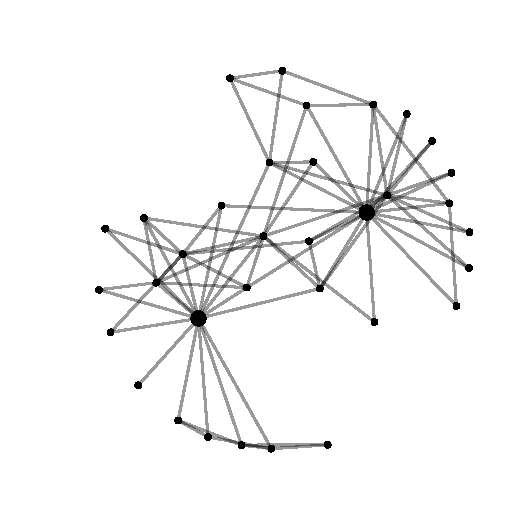
\includegraphics[width=.8\textwidth]{karate.pdf}%
\caption{Visualization of the karate network based on the data from \cite{10.2307/3629752}. The network is visibly structured around the two hubs 
(larger nodes), with clustered communities around each hub and a few nodes acting as intermediaries between the two communities.}
\label{fig:karate}
\end{figure}

As new algorithms attempted to find the most optimal division of the network in communities, it 
became therefore necessary to develop a method able to grasp the quality of the partition of the network. Among the various methods, the most popular one is the one of \textit{modularity optimization} \cite{Fortunato201075}.
This method, introduced by Girvan and Newman in 2002 \cite{Girvan11062002} is based on the idea that a good partitioning maximizes the amount of edges within a community and minimizes the amount of links towards the outside of the community. 
Modularity is therefore calculated as the difference in number of edges within a cluster and the expected number of edges that one would found in a similar network in which
individual nodes retain their degree, but the edges are randomly rewired. In Publication III a similar idea was used to investigate how dense the subgraph of Ego Networks, the graph formed by the neighbours of a specific individual (the ego) and by their mutual relationships, is. 
The EN is the realistic, local perspective of a given node representing the information that it might use in basic decision processes.
We calculated for new nodes joining the EN the fraction of references that stay within the EN, thus quantifying how modular the EN is and
how its modularity evolves in time. We showed that the EN has a sharp initial growth in modularity that saturates within 10 years,
before gradually decreasing as shown in Fig.\ref{fig:ego_modularity}.

Unfortunately, despite its simplicity, modularity also offers some limitations. Fortunato et al. showed in 2007 that modularity optimization is bound to have a resolution limit, i.e. a minimum size
of communities under which the method fails to detect communities \cite{Fortunato02012007}, which can represent an issue as real networks can be organized 
in hierarchical or tree-like structures  \cite{10.1371/journal.pone.0011976}. Furthermore, such resolution limit depends on the size of the network; as a network increases in size
the null model might expect two clusters to have a very low probability to be connected, therefore allowing one single connection between them to be seen as a strong
statistical indicator of modularity, thus merging the two clusters.
Even by trying to introduce a resolution parameter in order to find clusters of various sizes, problems such as merging of subgraphs and splitting
of graphs arise \cite{PhysRevE.84.066122}. Furthermore, another key limitation is the presence of multiple suboptimal solutions \cite{PhysRevE.81.046106} that still offer good results. While other methods are being introduced
with good results, they all come at a cost somewhere, due to the intrinsic loose definition of a community, thus forcing the scientists to perform a trial and error analysis based on the cumulative 
information gathered in the process \cite{Fortunato20161}. To summarize, there is no "Free Lunch" in community detection \cite{Peel2017}.
    
 \begin{figure}[h]
\centering
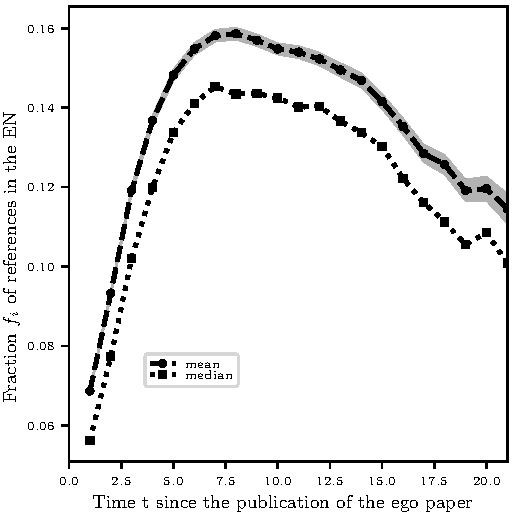
\includegraphics[width=.8\textwidth]{ego_modularity.pdf}%
\caption{Time evolution of the mean and median of the fraction $f_{i}$ of references of papers of the full Ego Network belonging to the Ego Network
as a function of the number of years since publication. In this framework, $f_{i}$ is the EN equivalent of the modularity of the community that is formed around the original paper. 
In the first years $f_{i}$ increases significantly, peaking after $ \approx 7$ years, after which a constant decrease takes place. Interestingly
however, the EN is also getting bigger in size, thus potentially allowing for more references to be part of the EN. Figure adapted from Publication III.}
\label{fig:ego_modularity}
\end{figure}

\section{Author networks}
As we have seen, network theory provides a solid framework with which to investigate social structures. It followed therefore that scientists could use the very same methods to investigate the social structure
of science itself. The main candidate for such analysis are author based networks, i.e. networks in which nodes are represented by individual scientists that are connected according to similarity in their publications.

The most straight forward approach is the one to considers co-authorship networks, in which links are assigned between scientists who collaborate in the writing of a single paper. The first study in the field was performed by Newman in 2001, by studying a dataset of over 2 milion papers and 1 milion authors in Physics, Computer Science and Biomedical research \cite{Newman16012001}.
This work allowed for the first time to quantify the collaborative structure of science with the newly formulated tools of network science. The data showed that the degree distribution, i.e. the number of collaborators
for a single author, follows a power-law behaviour with an exponential cutoff, a result coherent with a power-law degree distribution, with the cutoff being due to a size restraint in the system. The author also reports
that the network of scientific collaborations shows a small-world structure, with authors being no more than five or six steps apart from each other. The network showed also an interesting tendency for authors to cluster,
even though this might be biased by the presence of papers written by 3 or more authors, which, by the network construction rules, create triangles in the network. Newman's work showed the intrinsic social nature of science as a network
of collaborating nodes, with a structure that is coherent with a PAM in which authors with most collaborations are more likely to collaborate with new scientists. However, from
a theoretical point of view, it fails to find an explanation for the coexistence of a  power-law degree distribution and the intrinsic community-based structure, a feature absent in the PAM. 

The matter was further analyzed by Barab{\'a}si et al. \cite{Barabasi2002590}, who confirmed the clustering nature of co-authorship networks with a caveat: clustering, as well as other
 key properties of the network, are time dependent, therefore providing only partial information about the true structure of the network. This work, while reinforcing a preferential-attachment approach to the evolution
 of co-authorship networks, once again introduces the matter of time in the exploration of properties of the scientific community. 
 
 It has been suggested that a major role in the temporal aspect of co-authorship networks 
 may reside in the evolution of the individual careers of the different authors \cite{Wagner20051608}. Sociological considerations \cite{Gursey} can support the hypothesis that the preferential attachment method, that is the 
 phenomenon by which authors with many collaborations are more likely to have new ones,
 is the the driving force only of collaboration only for scientists in the middle of the career (thus also in the middle
of the distribution). The tails of the distribution instead are dominated by either established scientists, who don't require to build up their network anymore, or newcomers who instead fail to act as attractors
 in the network. It therefore follows that one cannot investigate the social structure of science in snapshots, but rather needs to follow its temporal evolution as  \textit{"networks
change over time, both because people enter and
leave the professions they represent and because practices
of scientific collaboration and publishing change"} \cite{Newman2004Connected}. 

Furthermore, one needs to step at a deeper structural level:
 while co-authorships provide the basic framework, it is important to differentiate between the various substructures that exist within a network as evidence shows that the local structure of the network
 has an impact on the citation and co-authorship patterns \cite{10.1371/journal.pone.0057546}. In fact, co-authorship practices are extremely heterogeneous across fields, as in certain applied sciences it is not rare
 to find papers co-authored by tens of authors, thus putting into question the ability of this approach to reflect the social structure of science. In fact, networks of different size need different collaborative behaviours for the 
 their community structure to persist in time. While smaller collaborative groups tend to be based on a core of strong relationships that are self-sufficient, larger groups need a more dynamic structure that
 reaches out to new members in order to survive, similarly to what happens in mobile communication networks \cite{Palla2007}. 

 Even though the co-authorship network is purely abstract in its formulation, it is possible to merge it with physical data, e.g. the location of the institution in which the authors work, allowing to add a 
 geographic dimension to the analysis. Relocation is common in academia, even though scientists usually are not likely to cover long distances, and can play a crucial role in one's career \cite{Deville2014}.
 Similarly, the choices of collaborators are also affected by geographical considerations that can be linked to policy making from individual countries or unions \cite{Hoekman2010662,Leydesdorff2008317}.


 
 \subsection{Ties and careers}
 In a framework in which the career and the connections of individuals change structurally over time, it becomes therefore fundamental to investigate the different nature of the links that connect different authors at different stages of their careers; after all science is not only
 driven by purely intellectual but also by more practical driving forces, such as economical and political matters that can also alter the paths of individual careers \cite{Kaplan2010,Petersen2012}, thus affecting
 the structure of collaborations both locally and in time. Similarly, as the network structures are known to influence team-performance \cite{Guimera2005,PentlandTeam}, it is natural to conjecture that these kinds of mechanisms are 
 reflected in the data of scientific collaborations. 
 
 In order to better understand such effects it is beneficial to investigate the role of the \textit{strength} of the ties between authors as a measure to identify which
 connections are more productive and represent a stronger tie within the sphere of scientific collaboration. This can be done by building a weighted network, where the weight of each link is defined as $w_{ij} =  \sum_{p} \frac{1}{n_{p} -1 }$
 where $p$ is the set of papers where authors $i$ and $j$ collaborate and  $ n_{p}$  is the number of co-authors of paper $p$.  
 Contrary to previous results in social networks \cite{Onnela01052007}, 
 collaborative networks show a unique characteristic: weak ties form the core structure of 
 dense neighbourhoods, with strong ties connecting different neighourhoods. This effect is considered
 to reflect the hierarchical and temporal dimension of scientific careers: as senior researches build strong ties with each
 other over time, they form research groups composed of young researchers \cite{Pan2012Ties,Ke2014}. Even though it is only
 a few strong links between senior scientists that keeps the scientific network of authors together, simulations show that 
 they are fundamental for the efficient spreading of information through the network. 
 
 In an academic world where
 most junior scientists drop out \cite{Pan2012Ties}, which is hierarchically and sometimes unequally structured in its hiring
 system \cite{Clausete1400005} and in which early developments can lead to a cumulative advantage in a career  \cite{MatthewEffect,Petersen04012011}
  it appears evident that the evolution of the social and collaborative structure of scientific interaction is closely related to 
 the evolution of the individual careers of the prominent scientists: their moving forward in the 
 hierarchy of science, projects their connections to a more important role within the scientific network and eventually allows them
 to influence the local properties of the network as they build their own team. 
 
 In 2015, Petersen published a work that offered an interesting insight
into the role of ties in the formation of careers and in their evolution  \cite{Petersen25082015}. In his longitudinal study of careers through an egocentric 
perspective of the collaboration network, the author found an exponential distribution in collaboration strength, allowing to define \textit{super ties} as
ties beyond a certain extreme threshold. Such ties appear to be equally distributed across disciplines(4\% of the collaborators are super ties), making
long lasting partnerships an intrinsic feature of scientific collaboration. Most importantly however, super ties were shown to have a positive effect
on individual careers as contributions to super ties are positively correlated with an increase in productivity in terms of numbers of publications, thus supporting
the growth of careers. Similarly, publications authored by super tie collaborators are statistically more likely to attract citations on the long term, receiving
on average 17\% more citations, probably due to an increase in visibility brought by the presence of a super tie collaborator.



 

\subsection{Centrality}\label{sec:centrality}
From the previous subsection we have seen that as junior researchers' careers unfold into
established academic positions and their early connections are carried along, they play a central role in the evolution of scientific network. 
But how can this property be measured? Once again, network theory comes to the rescue with the concept of \textit{network centrality}, thanks
to the computation implementation \cite{Newman200539,doi:10.1080/0022250X.2001.9990249} of basic ideas and algorithms originally introduced
decades earlier in the early years of quantitative sociological studies of social networks \cite{10.2307/3033543,Katz1953}.
The most common type of centrality is betweenness centrality \cite{10.2307/3033543}, which quantifies the centrality of node $j$ by calculating the number of shortest paths
between any two other nodes that goes through node $j$. A similar definition is the one of eigenvector centrality, which is based on a recursive idea
that that a node is central in the network if it is connected to other central nodes \cite{doi:10.1080/0022250X.1972.9989806}. 
Let $a_{ij}$ be the adjacency matrix of a graph. The eigenvector centrality $x_{i}$ of node $i$ is given by: $$x_i = \frac{1}{\lambda} \sum_k a_{k,i} \, x_k$$ where $\lambda \neq 0$ is a constant
and $a_{i,j}$ are the elements of the adjacency matrix and $\lambda$ is a constant. This score therefore recursively increases the score of a node if it is connected
to other nodes with high score, with the score being eventually measured in terms of degree.
This recursive equation can be solved by writing it in matrix notation and solving the eigenvector equation \cite{Ruhnau2000357} $$\lambda x = x A.$$

Eigenvector centrality can come in many forms \cite{Katz1953} and is also
the main idea behind Google's PageRank algorithm \cite{page1999pagerank}. Regardless of the practical definition of centrality, most of the measures are found to be strongly correlated with each other, with strong
values linked to a higher possibility to influence the flow of information through the network \cite{Valente2008}.

Data shows that the values of centrality in co-authorship networks are extremely skewed, with scientists with the highest score being
well separated from the 2nd tier, which in turn is well separated from the 3rd and so on, thus confirming the hierarchical structure
of science \cite{Newman2001}. Also, the weighted network analysis shows that within one's collaborators, there is a strong difference in how they contribute to the short paths, with 90\% of these paths
going through the top 2 collaborators, therefore reinforcing the idea of strong ties between the most relevant scientists.

Centrality measures therefore represent an excellent indicator of the absolute
importance of a scientist in the web of scientists, to the point where centrality itself can be shown to act as an attractor in models of preferential attachment  \cite{Abbasi2012403}. Authors who lie in
the center of network are therefore not only crucial for information spreading within the network, but also act as dominating actors who gather more attention than others to the point where the central positions
allows also to have a positive effect on citations count, which are strongly correlated with centrality measures \cite{Abbasi2011594,Sarigol2014}.





\section{Publication-based networks}
In Section \ref{sec:Citation Distributions} we discussed the distribution of citations, which in the paper based network framework represents the analysis of the in-degree distribution. However,
the structure of the connection between scientific papers can offer much more than a simple analysis of its properties.
In Publication III, we focused the analysis of the connections with papers from the point of view of the community that builds around a single paper. This kind of network is called an Ego Network (EN) and it has been extensively studied in social contexts \cite{mcauley2012learning,arnaboldi2012analysis}.
In a social network where nodes are individuals, those who are part of th EN are the ones that influence the most the Ego, as they form the community in which the Ego lives. Similarly, the EN of a scientific paper
is made by the set of all papers citing the Ego and of all the mutual citations between them. Fig.\ref{fig:EN} shows an example of an EN and of its evolution in temporal snapshots based on different time windows. The figure
shows a typical pattern of the EN. The EN is initially extremely dense, with initial citers being likely to be connected to each other. The density of the EN peaks after a few years, with the building of a strongly connected core while, however,
islands of isolated papers start to appear and eventually, after 5-10 years, the EN becomes extremely sparse. Interestingly, the global EN continues
to grow, indicating that later papers are also citing papers from earlier windows. This indicates that, despite the original idea of the Ego being still highly considered in the scientific community,
it fails to act as an aggregator of it, suggesting a specialization of the topic or, but not mutually exclusively, an increasing popularity of the ego in different disciplines.


\begin{figure}[htpb!]
\centering \large
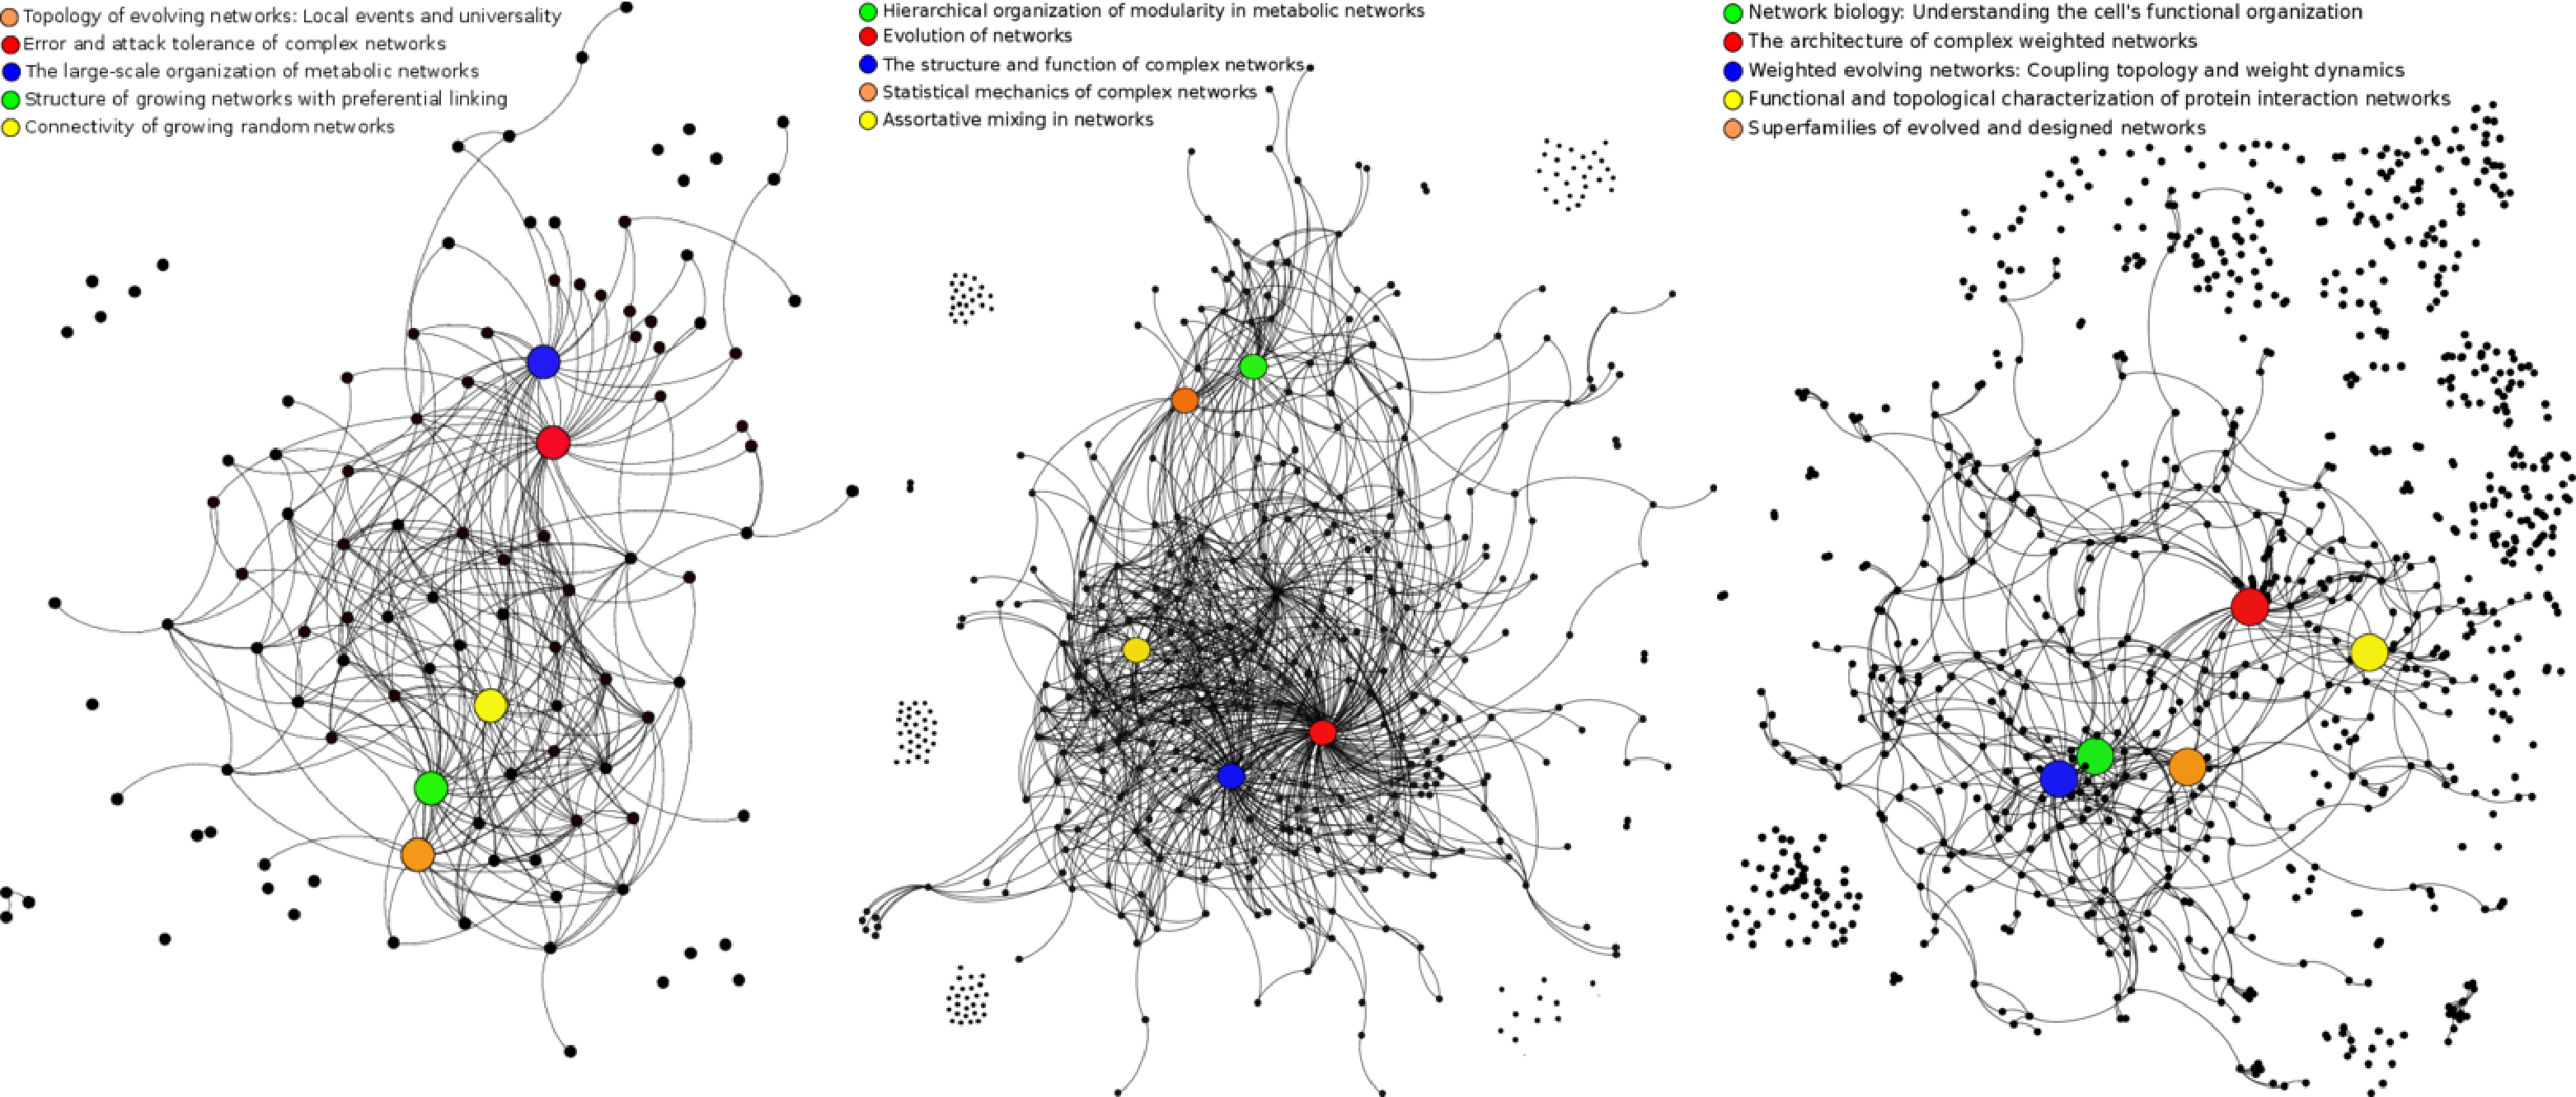
\includegraphics[width=\linewidth]{Figures/EN.pdf}

\caption{Ego-network for Barab\'asi and
R. Albert's  paper on scale-free networks \cite{Barabasi509}. We consider windows of size $w=2$ at $t$=1 (left), $t$=3 (center)
and $t$=5 (right), where $t$ is the number of years from
publication. Therefore the windows are non-overlapping and cover the
intervals 1-2, 3-4 and 5-6 (years after publication).
The EN is initially well connected, its link density is highest at
t=3, but it quickly becomes sparse, with a growing number of isolated
nodes. Some well known papers are highlighted with colors, their
titles are reported at the top. Figure adapted from Publication II.}
\label{fig:EN}
\end{figure}

While the EN approach aims at analyzing the local structure of the community around an idea/publication and its evolution in time, it is possible to
continue the analysis by "zooming out" gradually from the EN network, encompassing more and more layers of citations.
Even though a single paper might not have a massive first layer (i.e. citation count), it can accumulate a vast offspring in following layers, thus spreading its influence
to a large portion of the scientific network. 

The growth of the influence of an idea can be studied in its evolution, assigning a stronger weight to nodes
that lie in the lower circles and thus allowing to quantify the size and shape of the \textit{wake} of a paper \cite{10.1371/journal.pone.0113184}. Interestingly,
high values of this metric are able to reveal groundbreaking results that do not have high citation counts, with in particular Nobel laureates appearing as authors
of some of the most significant papers. In Publication IV we found a similar pattern: we introduced
a measure of the impact that a single paper has on the whole future corpus of science by allowing citing papers to "inherit" the scientific importance
of the cited paper. By recursively applying the method we are thus able to measure the global contribution of a paper in the scientific network and to compare the 
performance of papers between citations and impact. Fig. \ref{fig:nobel_impact} shows this comparison through a parameter $\delta = \frac{R_{c} - R_{i}}{R_{i}}$, where 
$R_{c}$ and $R_{i}$ are the rankings based on either citations (the former) or influence (the latter). $\delta$ measures
the outpferformance in impact vs. citation rankings, which is extremely high for Nobel papers if compared to papers with similar citation counts, thus
confirming that the cumulative importance "down the road" of scientific discoveries is not necessarily correlated to the first approximation, i.e.
the citation count.

\begin{figure}[h!]
\centering \large
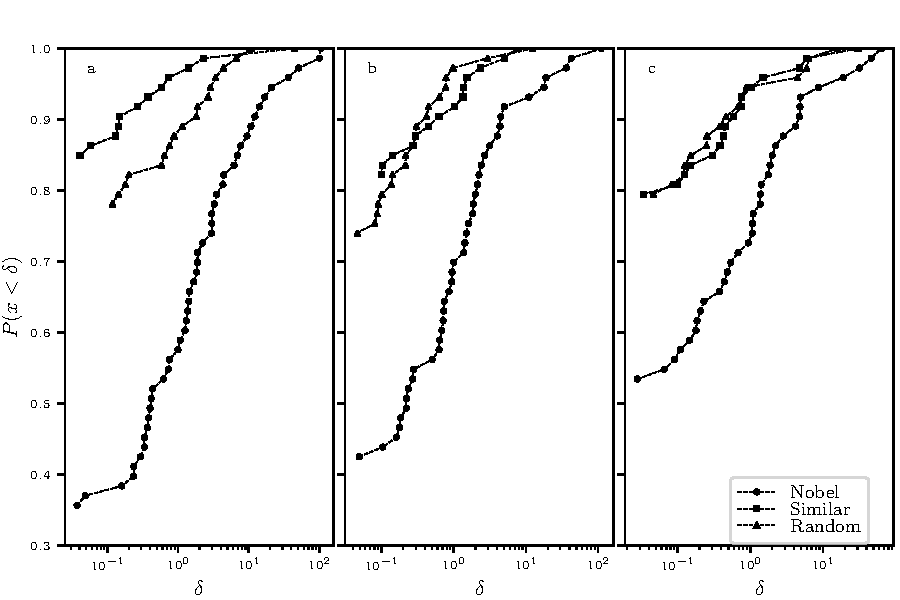
\includegraphics[width=.8\linewidth]{Figures/nobel_ranking_nCit.pdf}

\caption{Cumulative distribution of $\delta$ for Nobel papers, paper within a $3\%$ in citation volume in the same time interval compared to Nobel papers and for random papers
after five years (panel c), ten years (panel b) and at the end of the process in 2008 (panel a). Only papers
with positive $\delta$s are included. Nobel prize winning papers are more likely to climb the influence rankings, while similar papers behave
similarly to random papers. Also, while the fraction of Nobel papers that is climbing the ranking is increasing as time progresses, the control group
shows no significant change. Figure adapted from Publication IV.}
\label{fig:nobel_impact}
\end{figure}

As the previous examples show, the network structure of science can be an excellent indicator of the spread of ideas within the network. 
This kind of analysis has already been applied with success at a country and institutional
level \cite{Borner2006}. In this kind of framework, publications can be seen as new ideas introduced in a existing network, 
that are initially "exposed" to contagion from previous and become later the very source
of contagion for future works. This kind of approach borrowed from epidemiology \cite{Christakis2012}
is well known to be a driving force of the spread of new ideas \cite{Bettencourt2006513} and of the emergence and diffusion of topics across
disciplines. Susceptible-infected epidemic models applied to article networks
show that the diffusion of new ideas over disciplines takes a long time with the incubation period ranging from 4.0 to 15.5 years \cite{Kiss201074}. 

Another way to look at this process
is by comparison with genetics, seeing scientific ideas as genes that replicate/propagate themselves
to new publications in order to survive, an idea originally introduced by Dawkins in his book \textit{The Selfish Gene} \cite{selfishgene}. The term he coined
for these replicating entities is \textit{meme} and it has become extremely relevant nowadays, with the explosion of similar phenomena online that 
behave in such a way \cite{Leskovec:2009:MDN:1557019.1557077}. However, as genes and viruses replicate themselves to survive, they inevitably
end up competing for the same resources, thus leading to the inevitable disappearance of some of them \cite{Weng2012}. A meme based approach to
the spreading of scientific ideas has been attempted with success \cite{PhysRevX.4.041036}, introducing a meme score that quantifies the tendency of a 
scientific idea (e.g. chemical formulas or technical terms) to be replicated in a publication through a citation. Not surprisingly, high meme scores
are found to be important concepts in science.


\section{Communities, fields and multidisciplinarity}

In the previous sections we talked about the global structural properties of scientific networks that can be determined from network theory. However, the opposite process
can also be done. In the section on modularity and communities we discussed how the knowledge of the underlying structure of a network can be useful in order to devise methods
to analyze it, similarly in science we are aware \textit{a priori} that science is structurally organized in fields. Even within a single institution, there are separate
faculties or departments, in which scientists work separate one from another, with each group focusing on different branches of science. Fields are a concept everyone is familiar with
as the classical division of science in major branches such as Physics, Mathematics, Biology, Economics etc. is commonly used also outside the academic world and also
the ISI has a list of 21 static fields (or rather categories) used to label all journals. 

This categorization is simplistic and efficient on a superficial scale,
but we know science to be a intrinsically dynamic world. Bibliometric studies \cite{WeiweiCui2011} and studies on the co-occurrence network of scientific terms \cite{10.1371/journal.pone.0054847} have shown
that fields themselves are not static, but rather follow a life-cycle that may contain branching or merging events. It appears therefore evident from these observations that also
fields need to be studied not statically, but rather dynamically and that the information we know from scientific fields can be used recursively to analyze their changes
in time. 

Once again, works from epidemiology have been successfully applied to the topic. In a SEIR epidemic model scientists start off
being Susceptible to a new idea (i.e. working in a related field), transition to being Exposed to it (i.e. they have found out about it), proceed to become Infected spreading the idea before ultimately Retiring. 
Empirical evidence shows that the population growth of fields can be modeled with success by this 
model \cite{Bettencourt2008}. 

However, these processes are not always smooth: in 1970 the philosopher T. Kuhn discussed this matter in his famous book \textit{The Structure of Scientific Revolutions
} \cite{Kuhn:1970}, in which he described the process by which scientific knowledge progresses as being composed of periods of staticity separated by abrupt changes caused by \textit{paradigm
shifts} that challenge the scientific consensus. These shifts are mainly driven by discoveries of new information that contradicts and falsifies previous theories
and methods, thus requiring collaborative effort from the scientific community in order to provide new theoretical explanations. One of the most classic examples can be 
seen in the foundational crisis of most scientific fields at the end of the 19th century when Darwin's evolutionary theory, G{\"o}del's works on coherence and completeness and the new theory of Quanta
caused dramatic earthquakes in Biology, Mathematics and Physics. All these events happened sharply with either the experimental observation of new phenomena or the publication
of new innovative work which ultimately leads to completely new fields being born in a relative short time. 

One can therefore look at structural changes in the organization of fields
themselves in order to identify what are the crucial moments in the development of a single field. Studies on the temporal evolution of fields show that successful fields
grow in size, becoming more dense. In particular, the relationship between the number of edges and the number of nodes follows a scaling law :
edges = A(nodes)$^{\alpha}$, where $A$ and $\alpha$ are constant. This process is accompanied by a topological
transformation in the structure of the author network of the field: initially the authors are clustered in separate communities that, due to the densification
of the network, end up merging and forming of a \textit{large connected component} of authors, a phenomenon that does not take place for pathological cases (e.g. cold fusion in Physics)
due to the innovative failure of the original idea \cite{Bettencourt2009210}. This results show that the forming of a field is structurally connected to the forming of a sort of social network of authors
around an innovative concept. This social network, shown to be dense, can therefore be used as a \textit{ground truth} in community detection algorithms in order
to identify these communities in the global network. 

In fact, the changes in the connections between scientists and the subsequent change in modularity within the network
can be used to accurately model the birth of new fields as a process of merging and splitting of author communities \cite{Sun2013}. On the other hand, the diverse nature of fields
and their change in time undermines the possibility to use static definition of fields as a baseline for community detection. The application of modularity maximization
algorithm to paper network in fact has found that communities found in this way show a wide range of structure, varying from being strongly clustered to being barely noticeable \cite{Chen2010278}.
Furthermore, fields themselves are not monolithic blocks, but rather can be organized in structured hierarchical layers; Physics for example, manifests in its 
own paper network a number of subfields that have different local structure, with smaller subfields being more self-referential and thus more modular \cite{Sinatra2015}. This is to be expected:
the larger the extent of a field (or subfield), the more it is bound to see a diversification of its ideas and the reciprocal contamination with other fields and subfields. This process
leads to the birth of \textit{interdisciplinarity} and \textit{multidisciplinarity}.

The hierarchical nature  of fields and the structural overlapping across subfields and fields has led to the necessity to use also alternative methods for community detection, such
as clique percolation techniques \cite{Herrera2010}. Interdisciplinarity is not only an inevitable phenomenon of overlapping between fields,
but in recent years it has shown to become an intrinsic part of the core of Physics, gradually becoming more and more relevant \cite{Pan2012interdisciplinarity,Sinatra2015}.
Multidisciplainarity is slowly increasing and it can be analyzed in terms of the flow of information across fields \cite{Porter2009}, a technique that has led to the possibility of determining
the stabilization of interdisciplinary fields, thus becoming new stand alone disciplines \cite{10.1371/journal.pone.0008694}.

In Publication IV we studied the diffusion of scientific credit through the paper network, by spreading the scientific value of seed nodes from a field/subfield/journal of a certain year through the network.
By collecting the diffused scientific value and merging it into the same groups as the seed it is possible to measure the flow of information across fields. We found that
fields retain their information exponentially in time and that the exponent regulating the decay is increasing in time, thus manifesting an increase in multidisciplinarity which, 
however, might be a consequence of the increased rate of publication. A renormalization of time similar to the one in Publication I shows that the trend of increased interdisciplinarity is 
actually reversed, as shown in Fig.\ref{fig:multidisciplinarity}. Interestingly, multidisciplinarity shows to be the field slowing down the most in its tendency to share information, probably as a consequence
of it growing to the level of a stand-alone discipline with increased levels of self-referentiality.


\begin{figure}[h!]
\centering \large
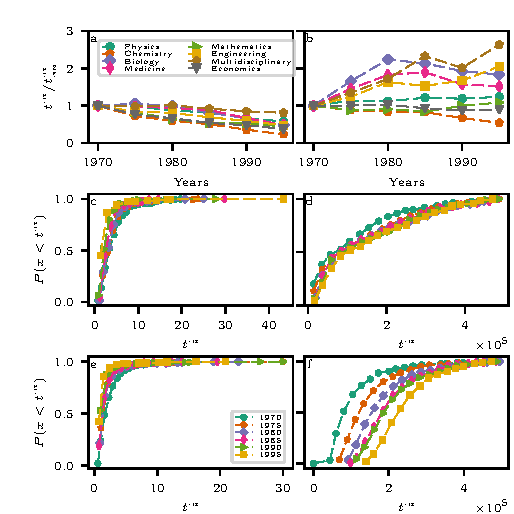
\includegraphics[width=.8\linewidth]{Figures/multidisciplinarity.pdf}

\caption{Changes in half life in time for the regular (left column, panels a-c-e) and renormalized scenario (panels b-d-f) and for different grouping of papers.
Panel a shows the evolution of the half life for a number of selected fields relatively to the 1970 value, in order to compare the trend across disciplines. We can see that fields
in general show a downward trend in which the half lives are decreasing. In panel b instead we can see the same evolution but but for the renormalized scenario, in which
time is measured in numbers of publications published. We can see that the trend either stabilizes or is reversed. Panels c and d shows the cumulative distribution of half lives for subfields and journals for 
different years, while panels e and f show the same distributions with renormalized half lives. We can see that the coloring order between the two columns is reversed, indicating
that also for subfields and journals are on average the same pattern as for the fields applies. Figure adapted from Publication IV.}
\label{fig:multidisciplinarity}
\end{figure}


